\section{Egenskaper i mottagare}
\index{mottagare!egenskaper}

\subsection{Selektivitet}
\textbf{HAREC a.\ref{HAREC.a.4.4.2}\label{myHAREC.a.4.4.2}}
\index{selektivitet}
\index{mottagare!selektivitet}

Med selektivitet menas en mottagares förmåga att skilja ut önskade
signaler och undertrycka övriga. Summariskt beskrivet kallas avståndet
mellan yttergränserna för det önskade frekvensområdet för
bandbredd. När det gäller superheterodynmottagare finns två
selektivitetsbegrepp.

Det ena är förselektering för att dämpa de spegelfrekvenser som
uppstår i samband med blandning av mottagna signaler och
oscillatorfrekvenser i mottagaren.

Det andra är selektiviteten i en superheterodynmottagares MF-steg som används
för att utskilja den önskade signalen efter blandningsförloppen.

\subsection{Spegelfrekvensproblemet vid mottagning}
\textbf{HAREC a.\ref{HAREC.a.4.4.5}\label{myHAREC.a.4.4.5}}
\index{spegelfrekvenser}
\index{mottagare!spegelfrekvenser}

\begin{figure}
  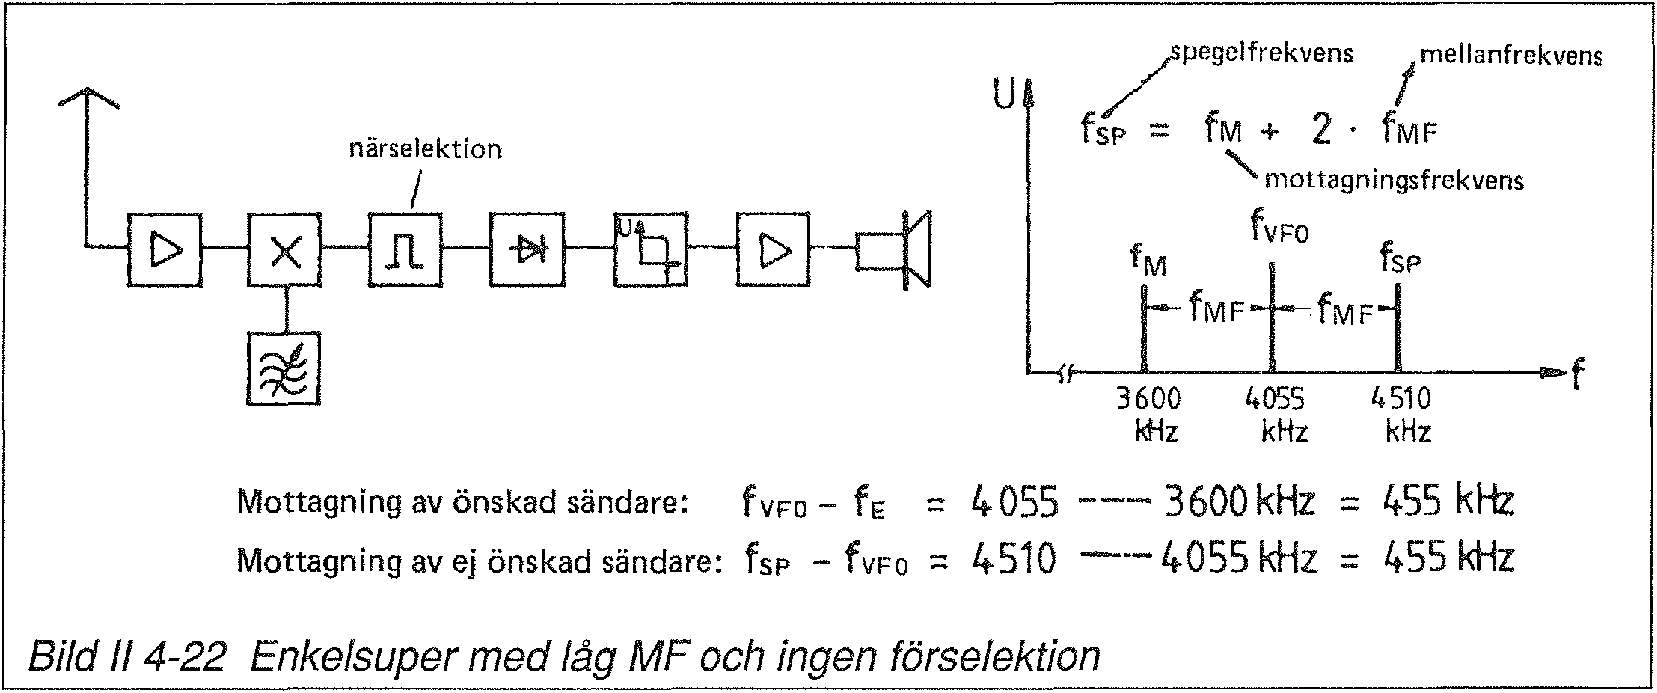
\includegraphics[width=\textwidth]{images/bild_2_4-22}
  \caption{Enkelsuper med låg MF och ingen förselektion}
  \label{fig:bildII4-22}
\end{figure}

Bild \ref{fig:bildII4-22}

Exempel: En sändning på 3600~kHz ska tas emot och VFO-frekvensen är
4055~kHz. Mellanfrekvensfiltret undertrycker sändningar på så
närliggande frekvenser som t.ex. 3603 och 3597~kHz. Denna egenskap
kallas för närselektion.

Men tyvärr kan en sändning på så avlägsen frekvens som 4510~kHz ändå
störa mottagningen, den goda närselektionen till trots. Avståndet
mellan 4510~kHz och vår mottagningsfrekvens 3600~kHz är 910~kHz.
Frekvensen 4510~kHz och VFO-signalen bildar också en
blandningsprodukt, som har frekvensen 455~kHz. Vid en VFO-frekvens av
4055~kHz och en mottagningsfrekvens av 3600~kHz benämns 4510~kHz som
spegelfrekvensen. Avståndet mellan spegelfrekvens och
mottagningsfrekvens är dubbla värdet av mellanfrekvensen -- i detta
exempel \(2 \cdot 455kHz = 910\) kHz.

Signaler på mottagningsfrekvensen och spegelfrekvensen alstrar båda
blandningsprodukter med VFO-frekvensen, som har mellanfrekvensens
värde. Mellanfrekvensfiltret kan därför inte undertrycka en främmande
signal på spegelfrekvensen.

\begin{figure}
  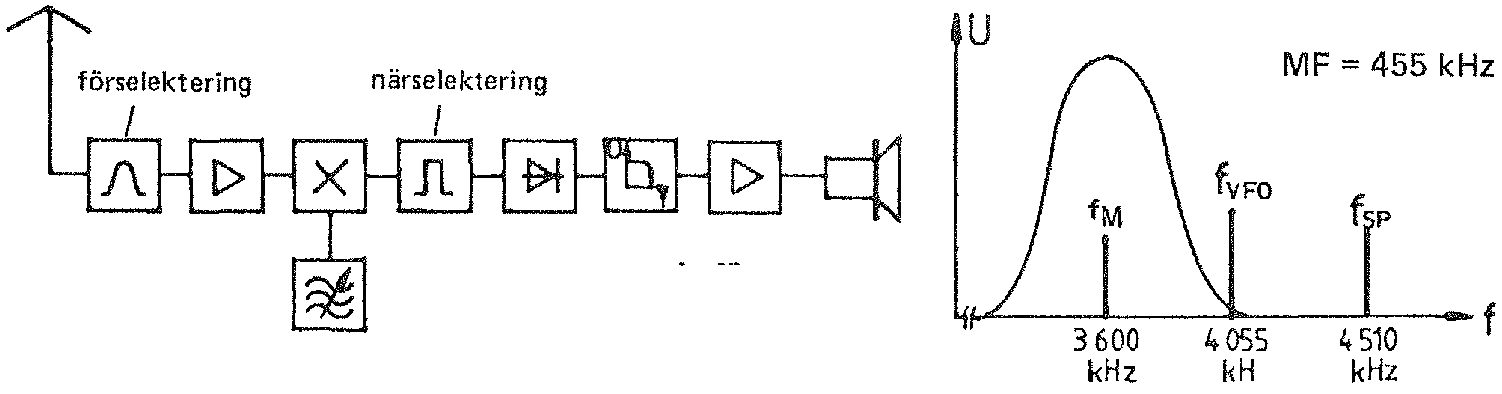
\includegraphics[width=\textwidth]{images/bild_2_4-23}
  \caption{Enkelsuper med låg MF och med förselektion}
  \label{fig:bildII4-23}
\end{figure}

Bild \ref{fig:bildII4-23}

Däremot kan en mottagaringång med förselektering undertrycka den. En
selektiv krets före blandaren släpper igenom ett smalt frekvensband
med mittfrekvensen 3600~kHz, men dämpar t.ex. frekvensen 4510~kHz
p.g.a. den stora frekvensskillnaden. En förselektion har alltså
tillförts som komplement till den närselektion som erhålls med
mellanfrekvensfiltret.

\begin{wrapfigure}{R}{0.5\textwidth}
  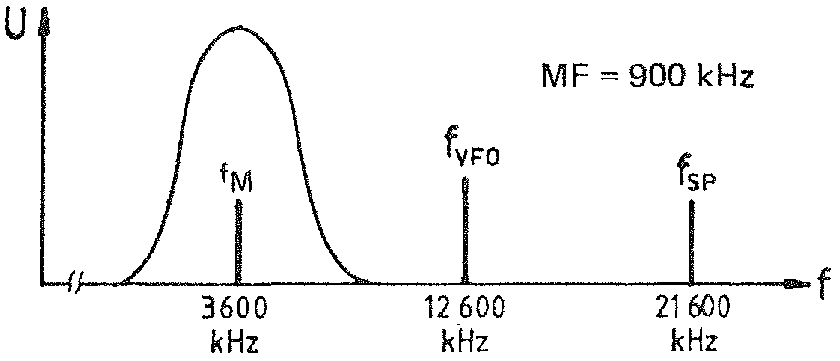
\includegraphics[width=0.5\textwidth]{images/bild_2_4-24}
  \caption{Enkelsuper med hög MF och med förselektion}
  \label{fig:bildII4-24}
\end{wrapfigure}

Bild \ref{fig:bildII4-24}

Ju längre ifrån varandra nyttofrekvens och spegelfrekvens ligger,
desto bättre är förselektionen. Med en mellanfrekvens av 455~kHz är
alltså detta avstånd 910~kHz. I långvågs- och mellanvågsområdet är det
tillräckligt för att man med enkla medel ska kunna skapa
tillräckligt selektiva filter.

Exempel: Vid den högsta mottagningsfrekvensen på mellanvåg 1605~kHz är
spegelfrekvensen 2515~kHz, som ligger 1,57 gånger högre i frekvens och
med ett avstånd av 910~kHz. I kortvågsområdet dämpas inte en
spegelfrekvens på avståndet 910~kHz tillräckligt kraftigt. Vid den
högsta mottagningsfrekvensen på kortvåg 30~MHz ligger nämligen
spegelfrekvensen 30,910~MHz endast 1,03 gånger högre i frekvens. Med
antagandet, att förselektionskretsen har ett Q-värde av 30, blir
bandbredden 53,5~kHz vid frekvensen 1605~kHz.

Med samma Q-värde blir bandbredden 1000~kHz vid frekvensen 30~MHz,
vilket innebär att förkretsen inte längre kan dämpa så närliggande
spegelfrekvenser på ett effektivt sätt.

I mottagare för högre frekvenser används därför högre mellanfrekvens
för att öka avståndet till spegelfrekvensen.
I moderna kortvågsmottagare är det vanligt med en mellanfrekvens av 9~MHz
eller högre.
Vid en mottagningsfrekvens av 30~MHz och en mellanfrekvens av 9~MHz är
spegelfrekvensen 48~MHz, vilket är 1,6~gånger mottagningsfrekvensen.
Detta möjliggör förselektionsfilter med tillräcklig dämpning av
spegelfrekvensen.

Bild \ref{fig:bildII4-25}

\begin{figure}
  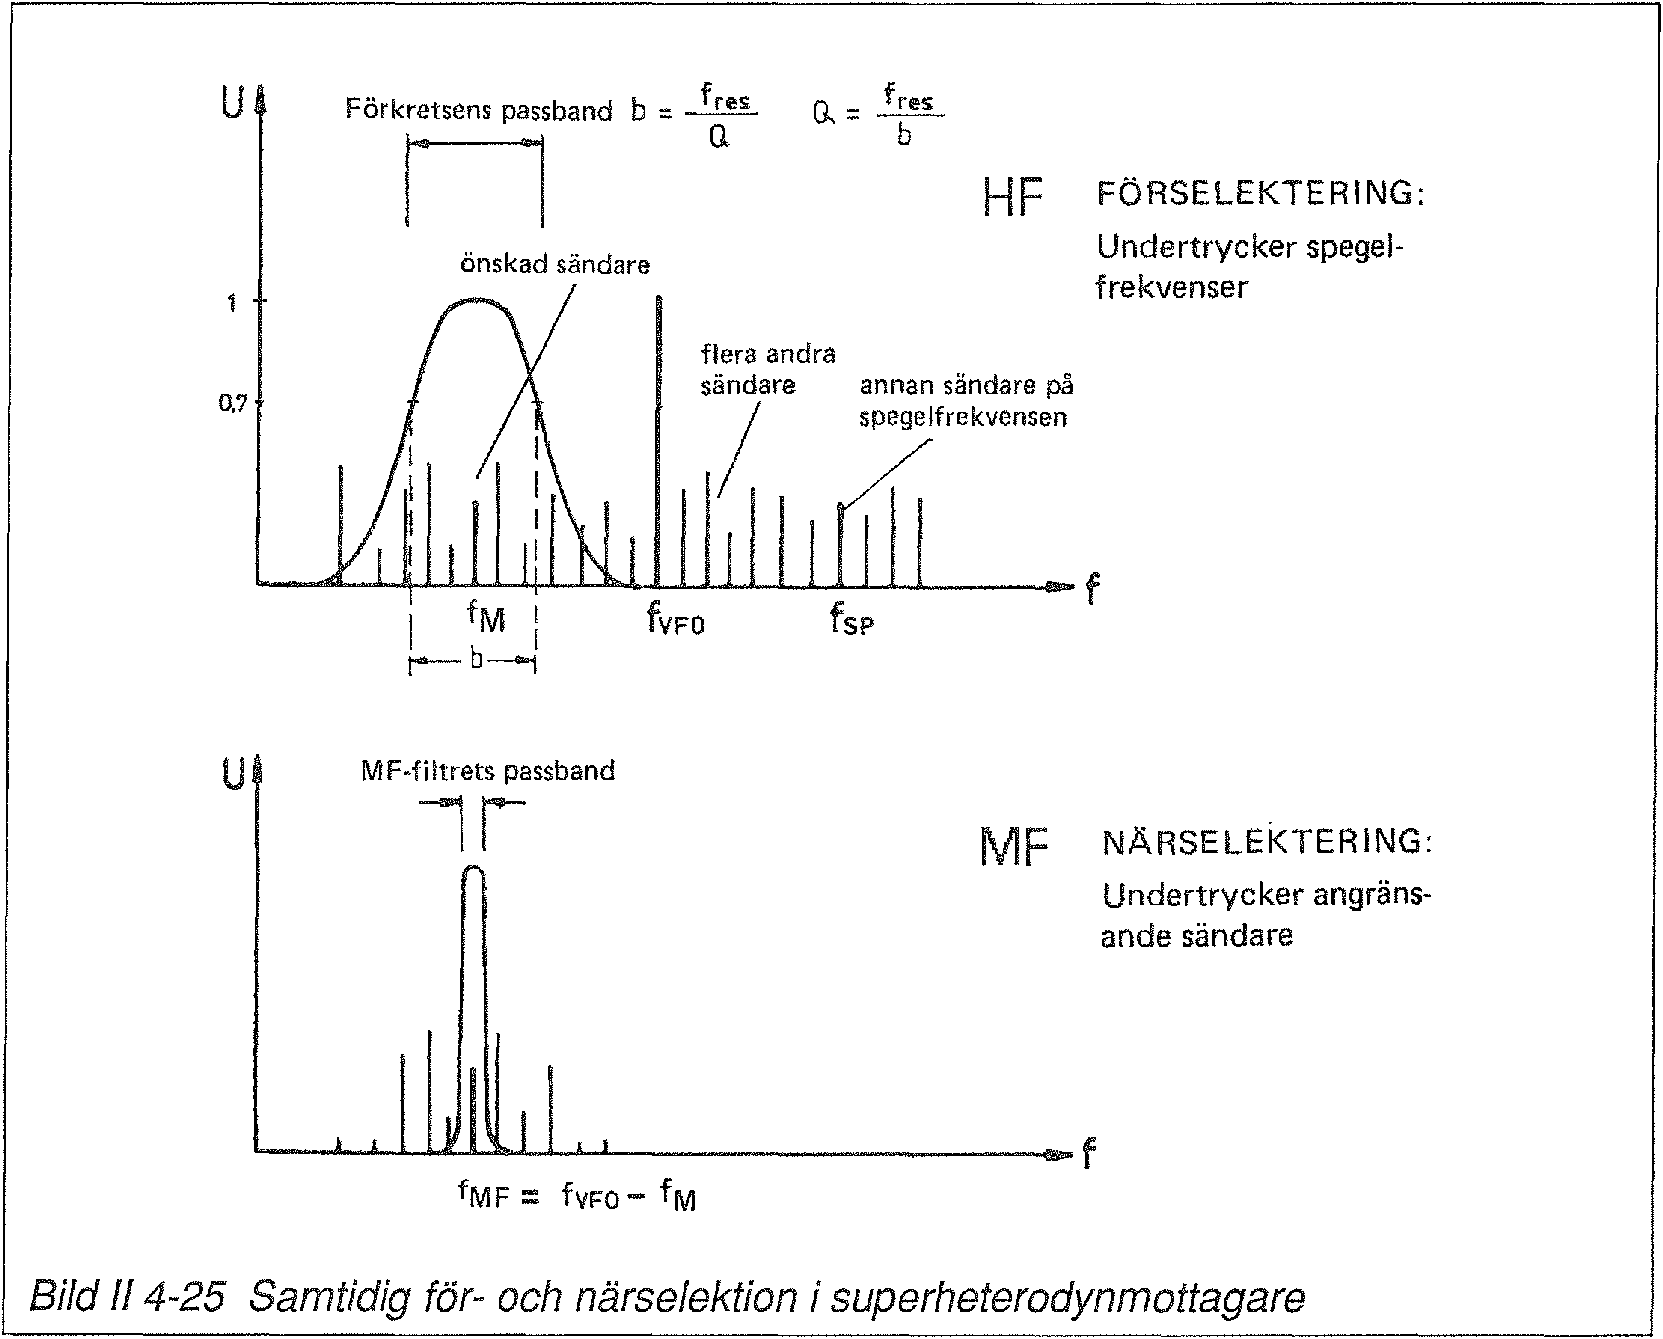
\includegraphics[width=\textwidth]{images/bild_2_4-25}
  \caption{Samtidig för- och närselektion i superheterodynmottagare}
  \label{fig:bildII4-25}
\end{figure}

Bilden visar hur när- och förselektion kompletterar varandra i ett
frekvensspektrum.  Märk, att passbandbredden \(b\) i
förselektionskretsen anger avståndet mellan de frekvenser där
signalamplituden dämpats till 70~\% av toppvärdet. I exemplet här ovan
har antagits att förkretsen för kortvågsmottagning har samma Q-värde
som förkretsen för mellanvågsmottagning.

Vid högre frekvenser, i VHF- och UHF-området, kan inte önskat Q-värde
erhållas i sådana kretsar som används i KV-området och lägre. Andra
lösningar blir då nödvändiga, t.ex. kavitetsfilter och helixfilter.

\subsubsection{MF-bandbredd vid AM (A3E)}
\index{AM}
\index{mottagare!AM}
\index{MF-bandbredd}
\index{mottagare!MF-bandbredd}

\begin{figure}
  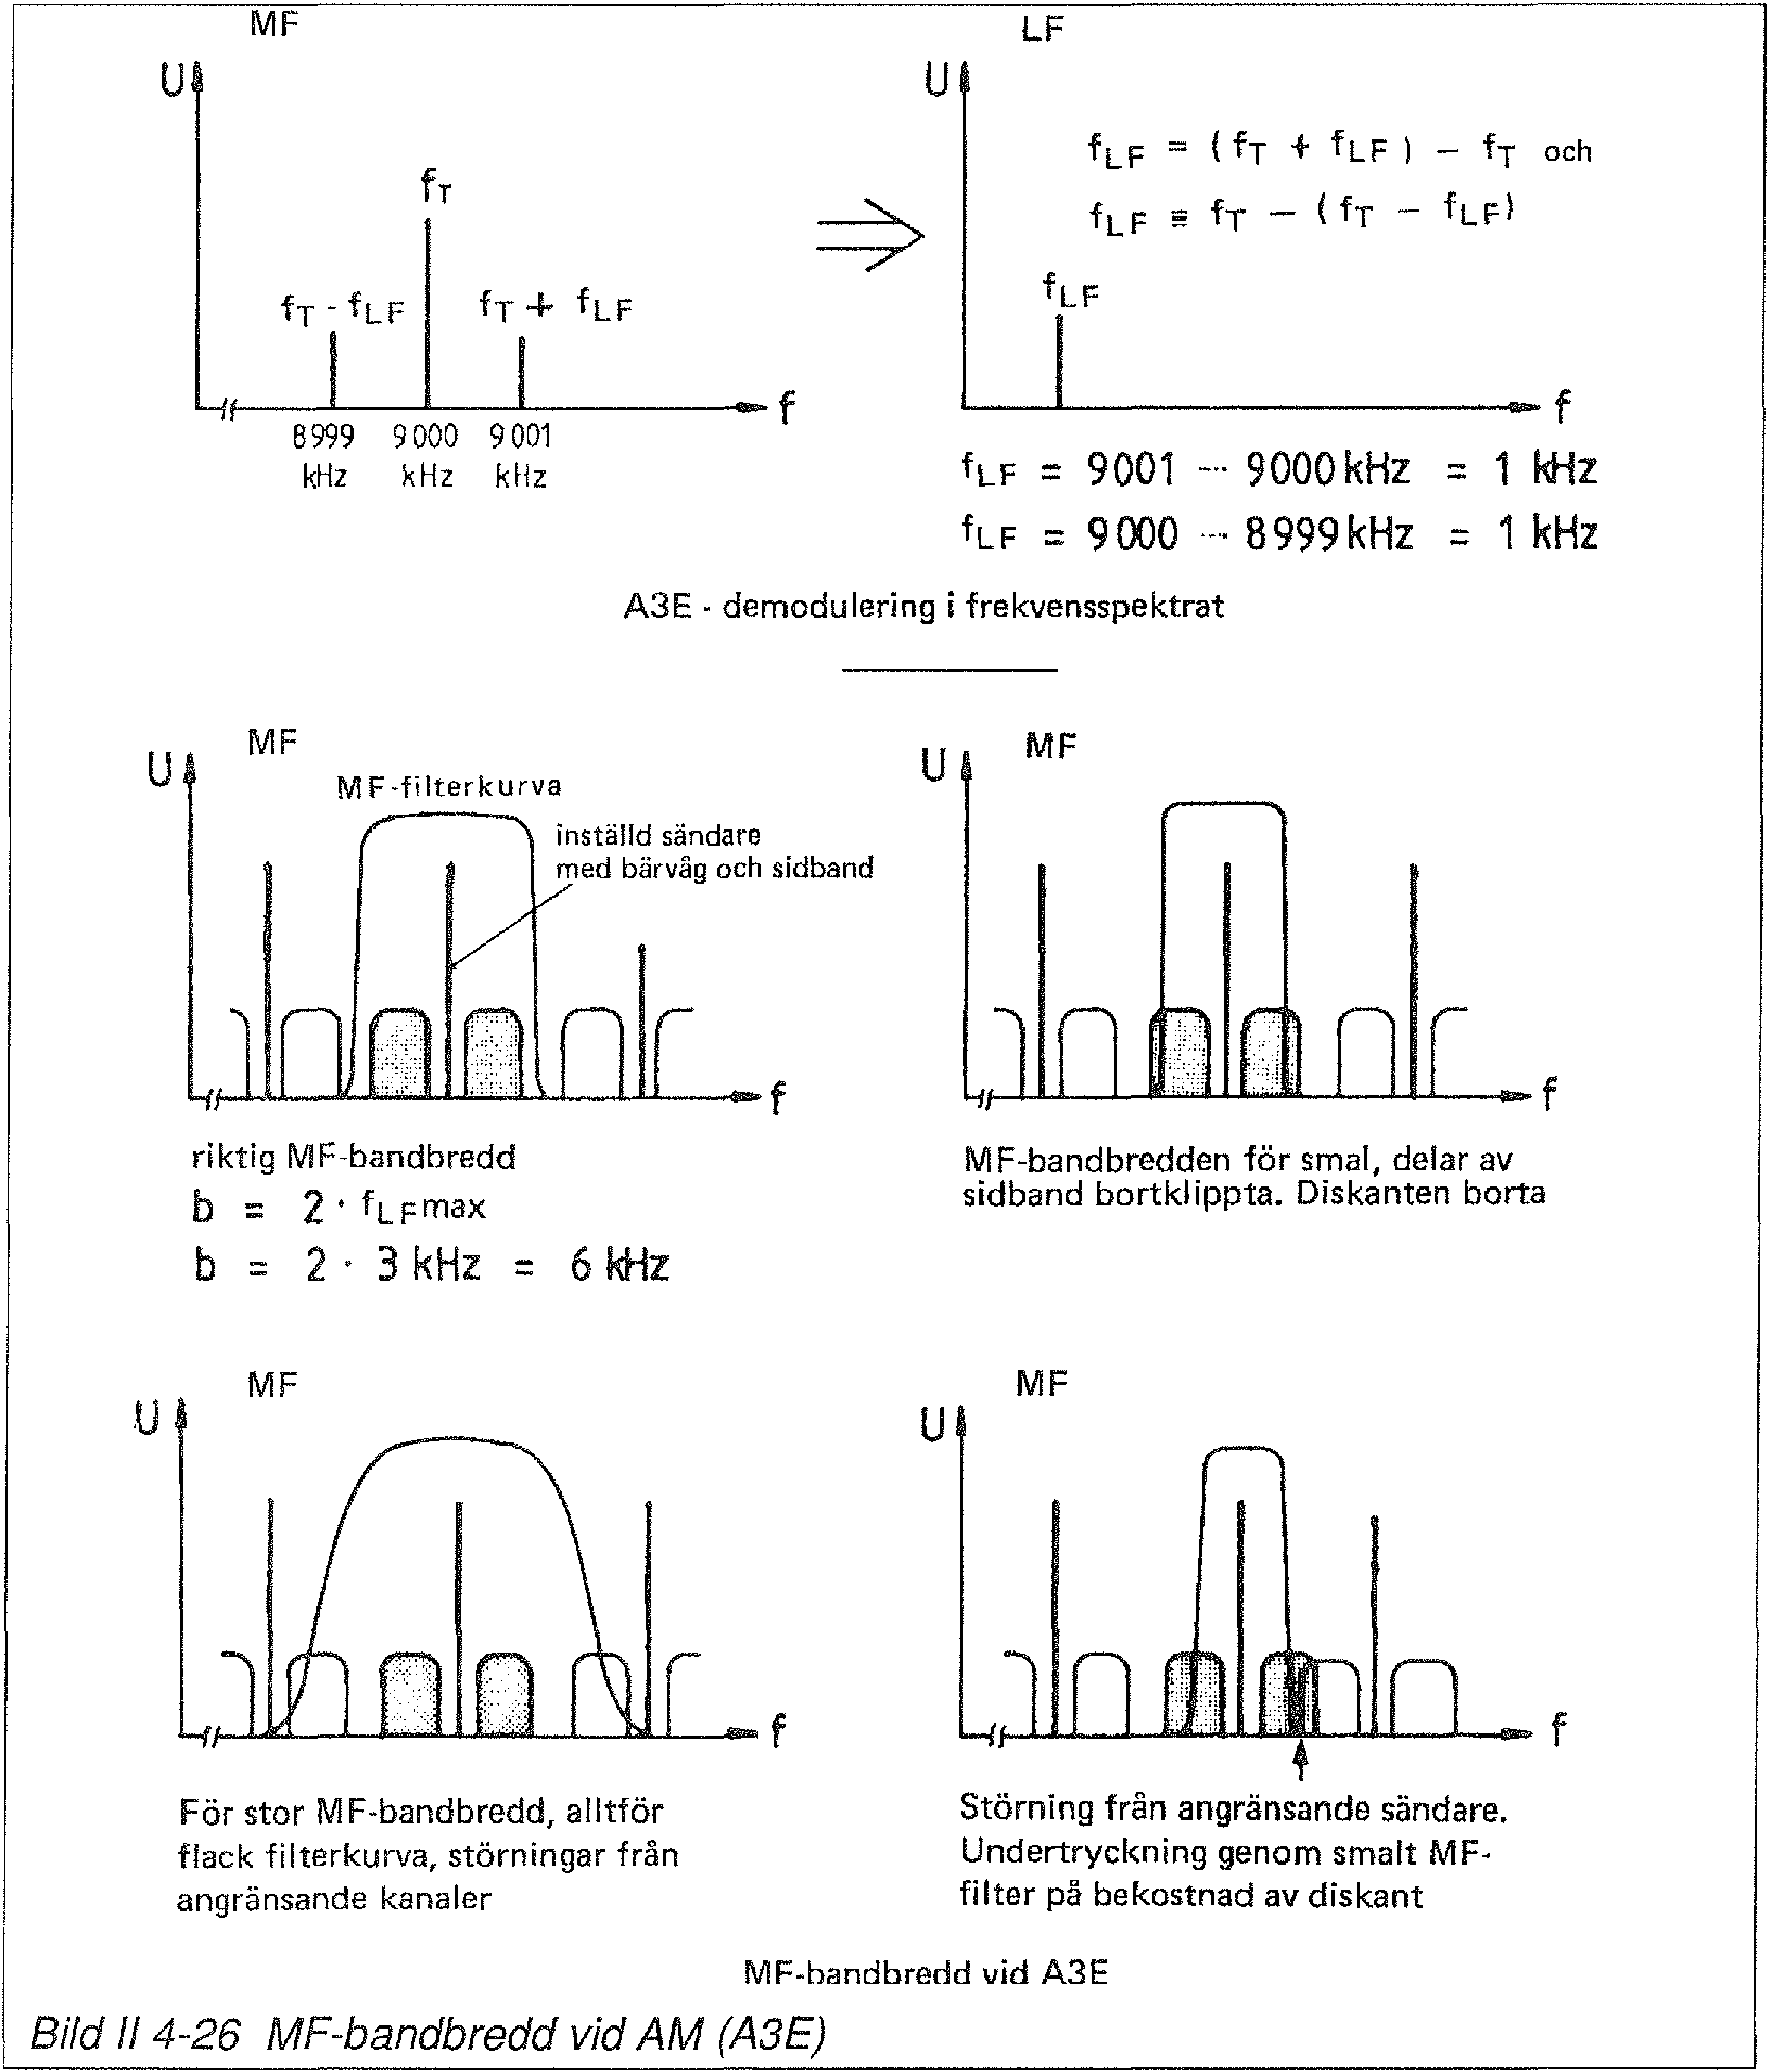
\includegraphics[width=\textwidth]{images/bild_2_4-26}
  \caption{MF-bandbredd vid AM (A3E)}
  \label{fig:bildII4-26}
\end{figure}

Bild \ref{fig:bildII4-26}

En amplitudmodulerad signals frekvensspektrum består av bärvågen och
två sidfrekvenser -- eller sidband om sidfrekvenserna är många.

Bandbredden i MF-kretsarna måste vara minst så stor att
sidofrekvenserna längst bort från bärvågen kan passera. Dessa
frekvenser motsvarar de högsta modulerande tonerna.
Vid rundradiosändningar på mellanvåg utsänds alla frekvenser upp till 4,5~kHz.
Detta motsvarar en bandbredd av 9~kHz. För enbart talöverföring
är en bandbredd av 6~kHz tillräcklig, vilket motsvarar en
LF-gränsfrekvens av 3~kHz.

Ett för smalt MF-filter skär bort de yttre delarna av
sidbanden. LF-signalerna kommer då att förlora de höga tonerna
(diskanten). Om däremot filtret är för brett, kommer närliggande
utsändningar också att höras.

I vissa mottagare kan MF-bandbredden anpassas till förhållandena. Det
är alltså en fråga om en kompromiss mellan bättre ljudkvalitet och
mindre störd mottagning.

\subsubsection{MF-bandbredd vid SSB (J3E)}
\index{SSB}
\index{mottagare!SSB}
\index{MF-bandbredd}
\index{mottagare!MF-bandbredd}

\begin{figure}
  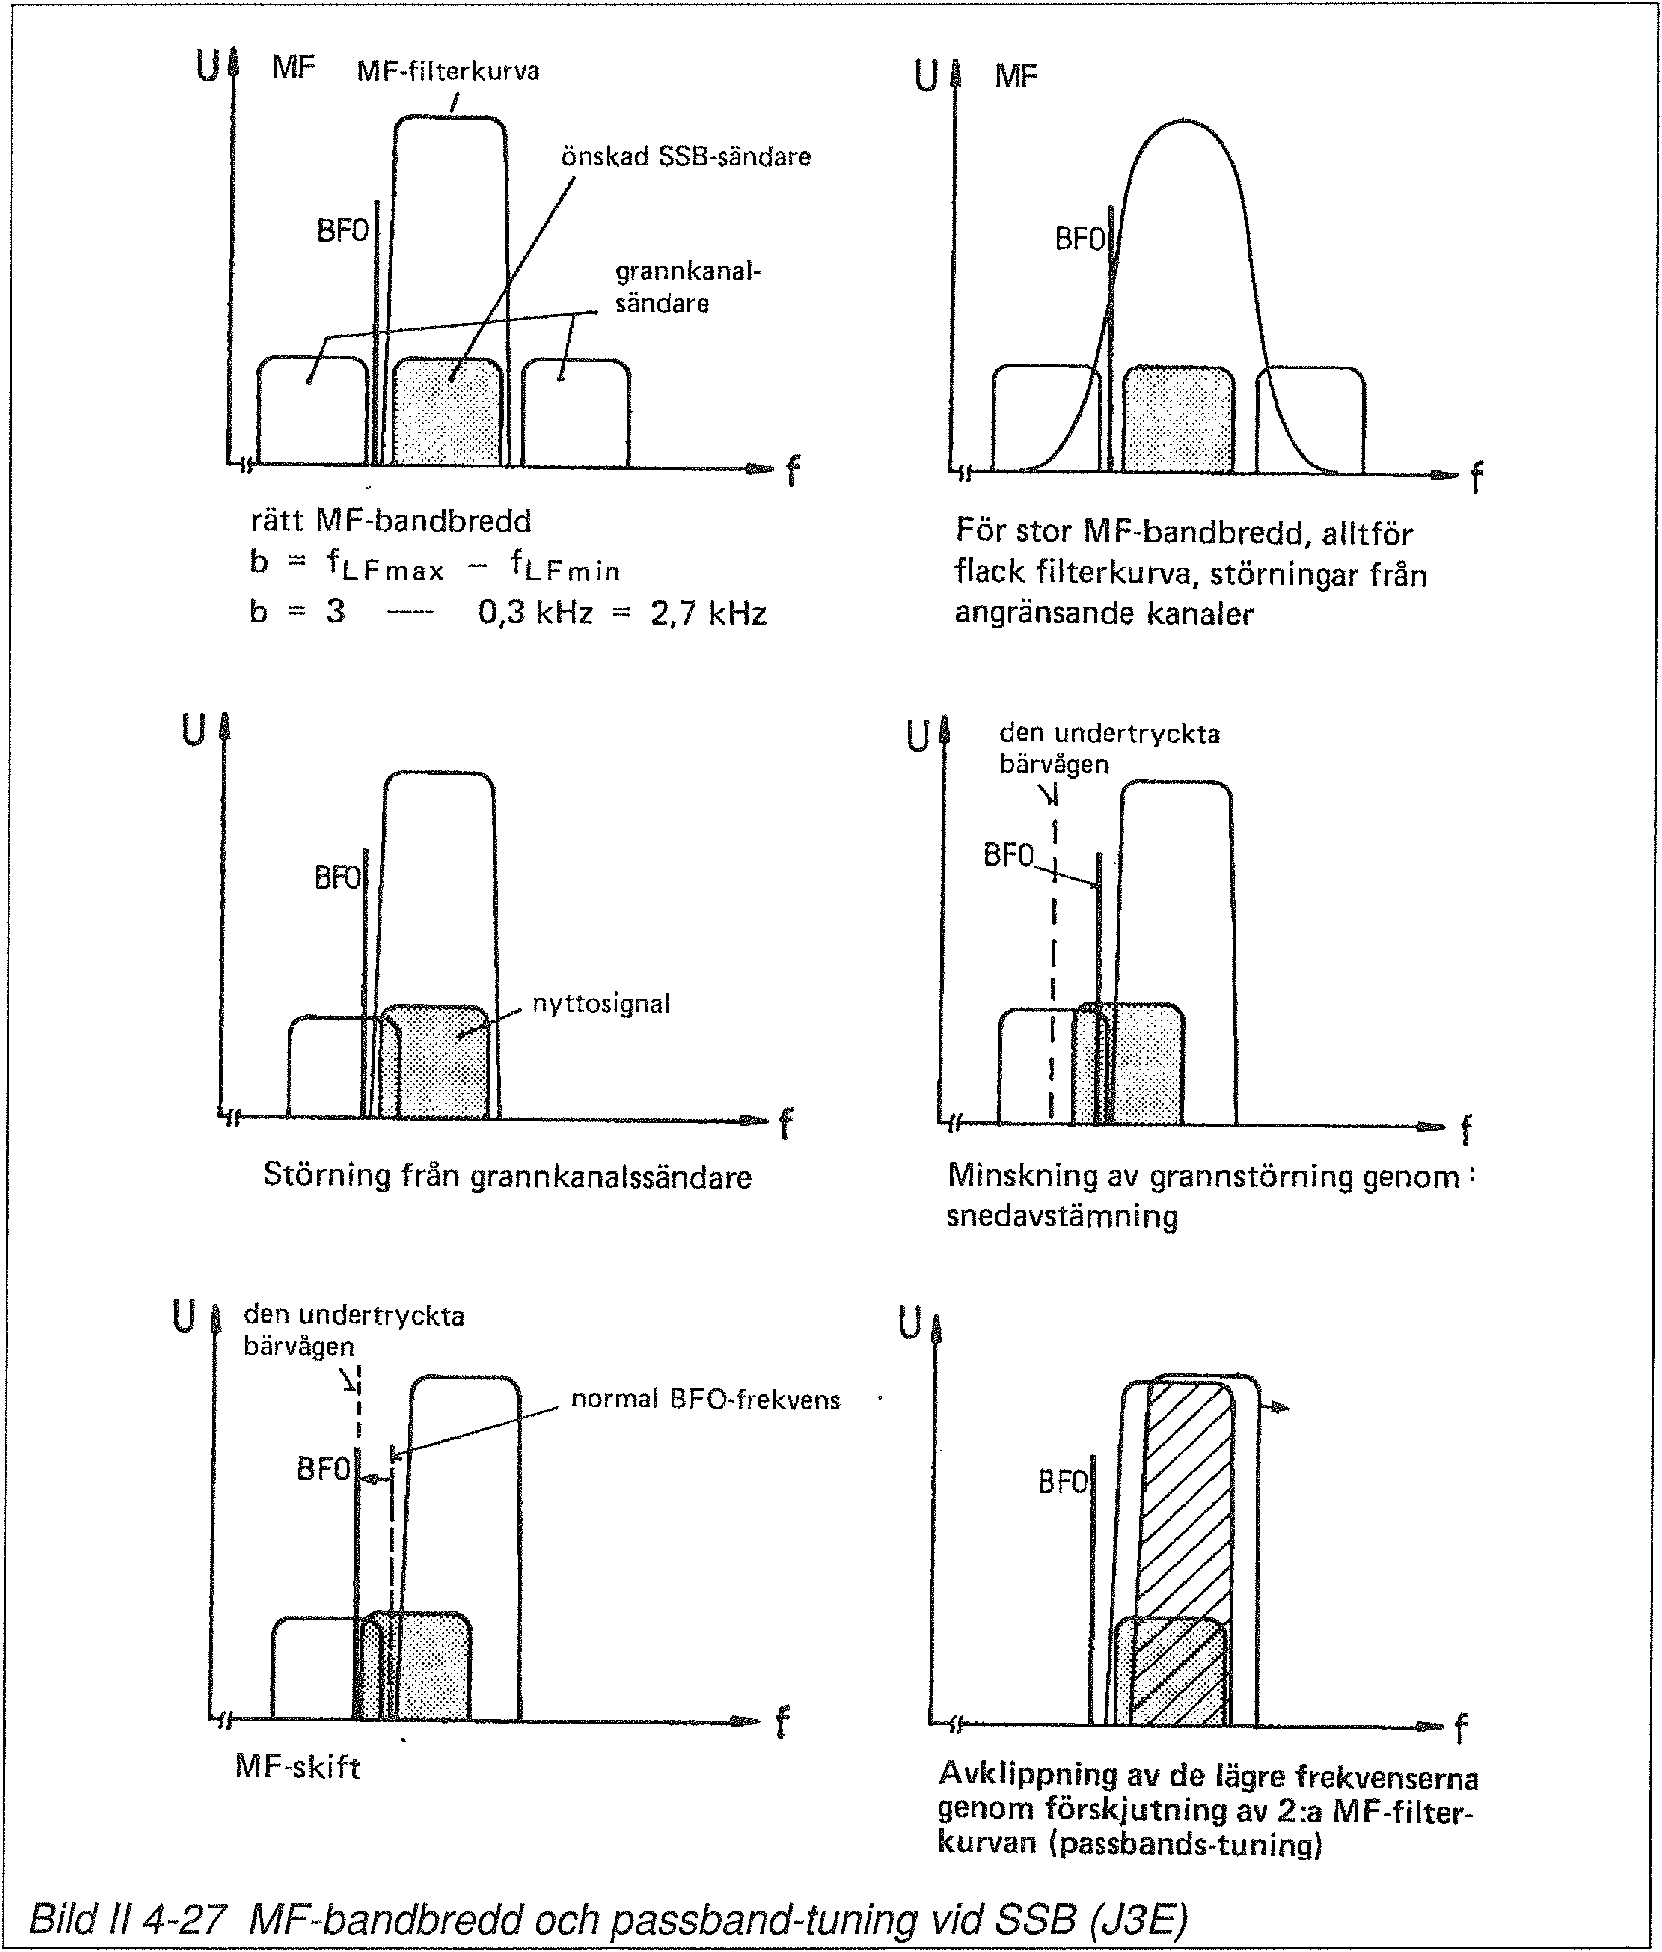
\includegraphics[width=\textwidth]{images/bild_2_4-27}
  \caption{MF-Bandbredd och passbandtuning vid SSB (J3E)}
  \label{fig:bildII4-27}
\end{figure}

Bild \ref{fig:bildII4-27}

Mellanfrekvensfiltret för SSB-mottagning ska endast släppa igenom
ett av de två sidbanden, vars bredd är skillnaden mellan högsta och
lägsta överförda LF-frekvens. Inom amatörradio är detta 3~kHz - 0,3~kHz
= 2,7~kHz, alltså något mindre än hälften av bandbredden vid AM.

Ett alltför brett MF-filter skulle också släppa igenom oönskade
signaler från angränsande frekvenser. A andra sidan skulle ett för
smalt MF-filter skära bort signaler i det önskade frekvensregistet och
försvåra mottagningen. Smala filter kan å andra sidan utnyttjas för
att dämpa signaler, t.ex. från en för nära liggande sändare eller en som
har för stor bandbredd.

När närliggande sändare stör mottagningen ges följande möjligheter:
\begin{itemize}
  \item Att göra en liten snedavstämning, uppåt eller nedåt i
    frekvens. Därigenom ändras frekvensläget på det mottagna talet,
    men vid små frekvensavvikelser blir förvrängningen
    liten. Läsligheten blir sämre, men mottagningen på det hela taget
    bättre.

  \item MF-skift. Som just beskrivits kan en liten snedavstämning
    göras. i vissa mottagare är det ordnat så att också BFO-frekvensen
    kan förskjutas så att frekvensläget på talet blir återställt
    igen. Därmed blir MF-passbandet skenbart förflyttat uppåt
    eller nedåt i frekvens (MF-skift, IF-shift).  Det verkliga
    frekvensläget mellan nyttosignal och BFO behålls. I alla händelser
    blir basen eller diskanten på nyttosignalen avskuren, beroende på
    var denna ligger i frekvens.

  \item Passband-tuning. Om det finns störande sändare både över och
    under i frekvens, går det inte att skära bort störningarna med ett
    enkelt MF-skift, eftersom antingen den ena eller den andra
    störande sändaren ändå skulle höras. För det fallet erbjuder några
    moderna mottagare möjligheten att flytta MF-passbandets övre och
    undre frekvensgräns oberoende av varandra (bandpass tuning
    m.m.). Detta förutsätter, att mottagaren är en trippelsuper med
    branta filter i varje MF-steg.  Vidare måste VFO, 1:a BFO och 2:a
    BFO kunna ställas in var för sig. Frekvensläget på MF I och/eller
    MF II kan då förskjutas över respektive filters passband,
    oberoende av varandra. Därigenom uppstår skenbart effekten att
    filterkurvorna skjuts emot varandra. Samma effekt skulle fås om
    kristallfiltren gick att avstämma, vilket ju inte är möjligt.
\end{itemize}

\subsubsection{MF-bandbredd vid CW (A1A)}
\index{CW}
\index{mottagare!CW}
\index{MF-bandbredd}
\index{mottagare!MF-bandbredd}

Bild \ref{fig:bildII4-28}

En CW-signal har som bekant inte bandbredden noll Hz, utan det handlar
i grunden om en amplitudmodulerad signal. Vid en nycklingshastighet av
60 tecken per minut är bandbredden ca 100~Hz och vid i 120 tecken per minut
den dubbla, ca 200~Hz.

I vissa mottagare används ett SSB-filter även för mottagning av CW. En
vanlig bandbredd på ett SSB-filter är 2,7~kHz och då kommer även
stationer på närliggande frekvenser att höras. Låt vara att de flesta
av dessa stationer hörs med olika frekvens.

\begin{figure}
  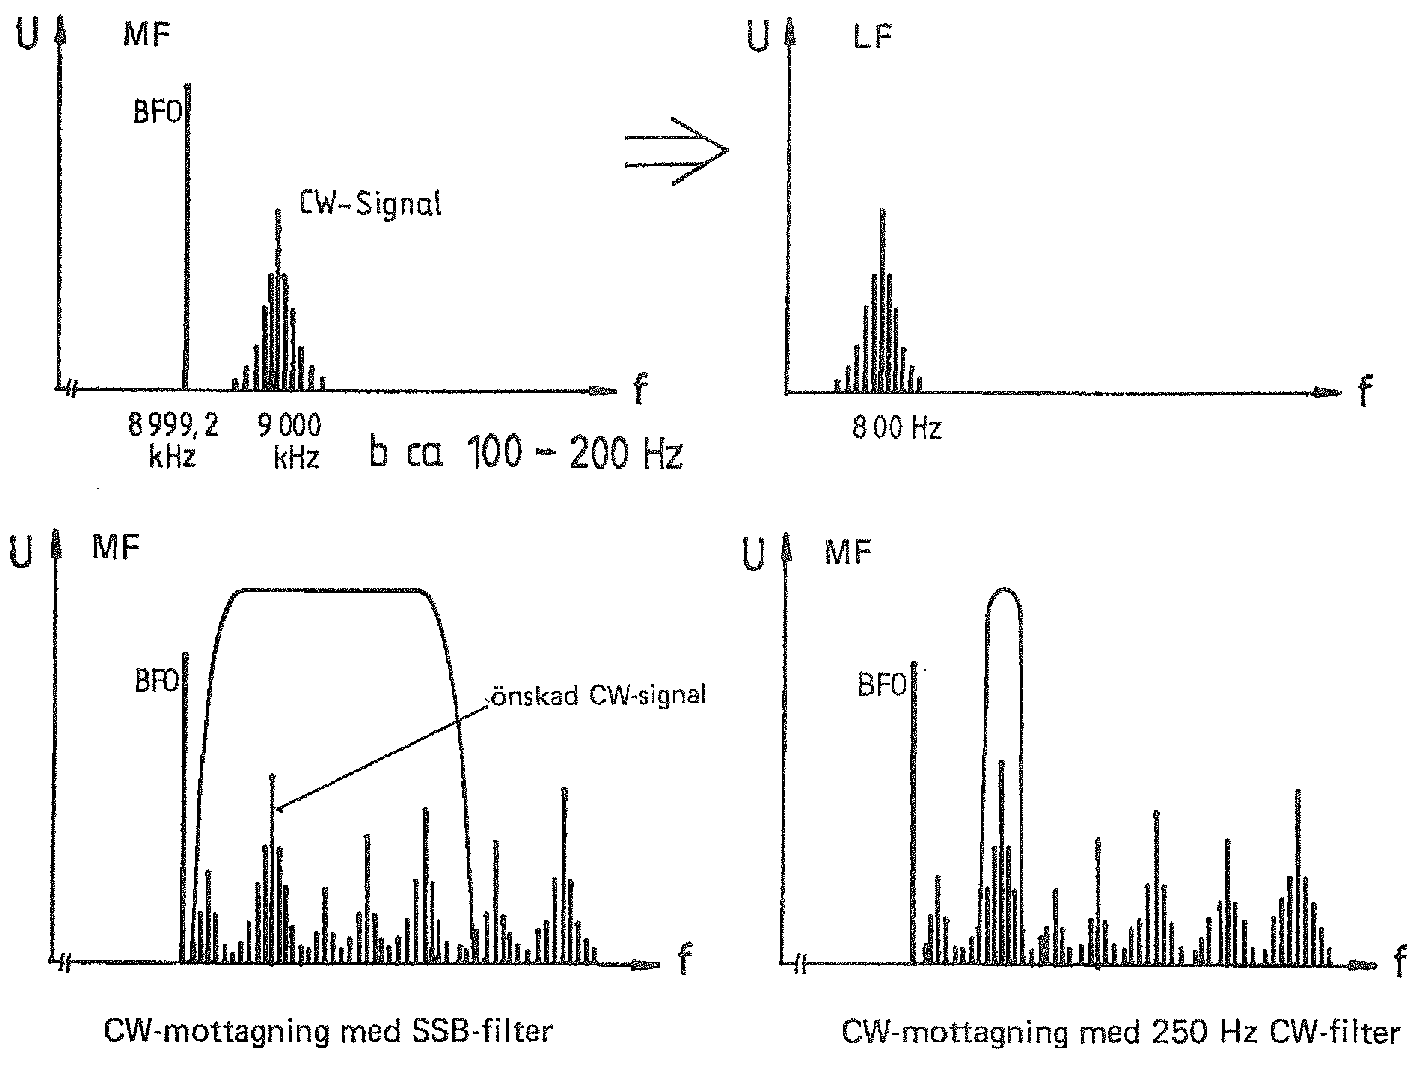
\includegraphics[width=\textwidth]{images/bild_2_4-28}
  \caption{Olika MF-bandbreder vid CW (A1A)}
  \label{fig:bildII4-28}
\end{figure}

Fler än 20 CW-stationer får plats inom en bandbredd motsvarande en
SSB-kanal. Den mänskliga hjärnan, kan med någon övning koncentrera sig
på en av dessa signaler medan övriga uppfattas som störande.

Det tidigare nämnda LF-bandpassfiltret skulle emellertid åstadkomma en
bättre selektion och bekvämare avlyssning. Men om en annan station
inom passbandet är mycket starkare än den station som är av intresse,
då blir MF-förstärkaren antingen överstyrd av den starkare signalen
eller AGC reglerar ner förstärkningen så att den svagare signalen inte
längre kan höras trots det smala LF-filtret. Selektionen i en
mottagare bör därför sitta ''så långt fram som möjligt''. I det
skildrade exemplet skulle ett smalt filter i MF vara till bättre nytta
vid CW-mottagning. Bandbredden på ett sådant filter är 250--500~Hz,
således endast något bredare än CW-signalen.

Med ett ännu smalare CW-filter kan, p.g.a. bristande
frekvensstabilitet hos sändare och/eller mottagare, svårigheter
uppstå att finna den önskade signalen. Välutrustade mottagare har
passband-tuning även för CW, steglös bandbreddsreglering eller stegvis
valbara filterbandbredder. Då kan mottagaren ställas in på den önskade
signalen med en stor bandbredd som därefter minskas.  För mottagning
av RTTY (radiofjärrskrift) med 170~Hz skift mellan de två
frekvenserna, kan ett 500~Hz-filter användas. Smalare filter går
däremot inte så bra.

\subsubsection{Bandbredd vid FM (F3E)}
\index{FM}
\index{mottagare!FM}
\index{MF-bandbredd}
\index{mottagare!MF-bandbredd}
\index{frekvensdeviation}
\index{bandbredd}

En FM-sändare med frekvensdeviationen \(∆f_{max}\) och högsta
modulerande LF-moduleringsfrekvensen \(f_{LF_{max}}\) har bandbredden

\[ b = 2 \cdot (∆f_{max} + f_{LF_{max}}) \]

Inom amatörradio är det brukligt med en maximal deviation av 3~kHz och
en övre gränsfrekvens av 3~kHz, vilket motsvarar en bandbredd av 12~kHz.

Fullgod mottagning är möjlig endast om MF-filtren i mottagaren har
minst den bandbredd, som sändaren har. Men vid för stor
mottagarbandbredd kan även stationer på närliggande frekvenser
uppfattas. Sedan 1996 är det av IARU Region 1 rekommenderade
kanalavståndet 12,5~kHz vid FM-trafik på VHF- och
UHF-amatörradiobanden.

Det är vanligare med för stor deviation på FM-sändaren än att
mottagaren är alltför smal. En för stor deviation, avsaknad av
deviationsbegränsare och för hög LF-gränsfrekvens medför en onödigt
stor bandbredd på sändaren. Motstationen får då mottagningssvårigheter
och stationer på angränsande kanaler blir också störda.

Det blir allt vanligare med 12,5~kHz kanalavstånd även för repeatrar,
varför det är viktigt att alla sändare är rätt inställda.

\subsection{Signalkänslighet och brus}
\textbf{HAREC a.\ref{HAREC.a.4.4.3}\label{myHAREC.a.4.4.3}}
\index{signalkänslighet}
\index{mottagare!signalkänslighet}
\index{brus}
\index{mottagare!brus}

Om man ställer in mottagaren på en ledig frekvens, så hör man vid full
förstärkning ett brus likt det från ett vattenfall.

Bruset kommer från de svaga växelspänningar som uppstår när
laddningsbärarna rör sig genom de material som strömkretsen består
av. Beroende av bruskällan sträcker sig frekvensspektrum från noll
till nära nog oändligt. På grund av egenskaperna skiljer man mellan en
rad specifika bruskällor:
\begin{itemize}
\item Resistorbrus, även kallat ''vitt brus'', som uppstår i resistiva
  komponenter. Bruset sträcker sig över hela det mätbara
  frekvensområdet varvid energifördelningen är lika över hela området,

\item Kretsbrus, som uppstår i resistanser i svängningskretsar i
  resonans,

\item Antennbrus, som är sammansatt av bruset från antennens
  strålnings- och förlustresistanser samt av det galaktiska brus som
  antennen tagit emot,

\item Transistorbrus uppstår av laddningsbärarnas rörelser i
  halvledarmaterial.
\end{itemize}

Det bildas en sammanlagd brusspänning som kan bestämmas. Man talar om
ett brustal, som är ett mått på mottagningssystemets egenbrus. Detta
ska ställas mot styrkan på den mottagna signalen. Man talar om ett
förhållande mellan signaleffekt och bruseffekt. Det finns flera
metoder att mäta och uttrycka detta förhållande som kallas S/N (signal
to noise ratio). För att uppfatta den information som kommer ur en
mottagares LF-utgång måste nyttosignalen vara ett antal gånger
starkare än bruset. Den lägre gränsen för att uppfatta tal i
kortvågsmottagare är ett brusavstånd i storleksordningen 10~dB.

\begin{wrapfigure}[19]{R}{0.5\textwidth}
  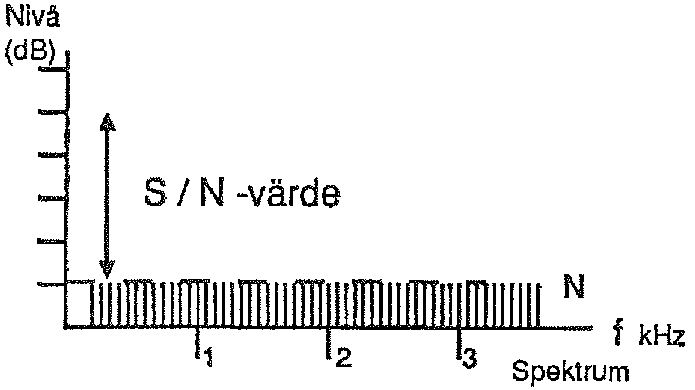
\includegraphics[width=0.5\textwidth]{images/bild_2_4-29}
  \caption{S/N-värde}
  \label{fig:bildII4-29}

  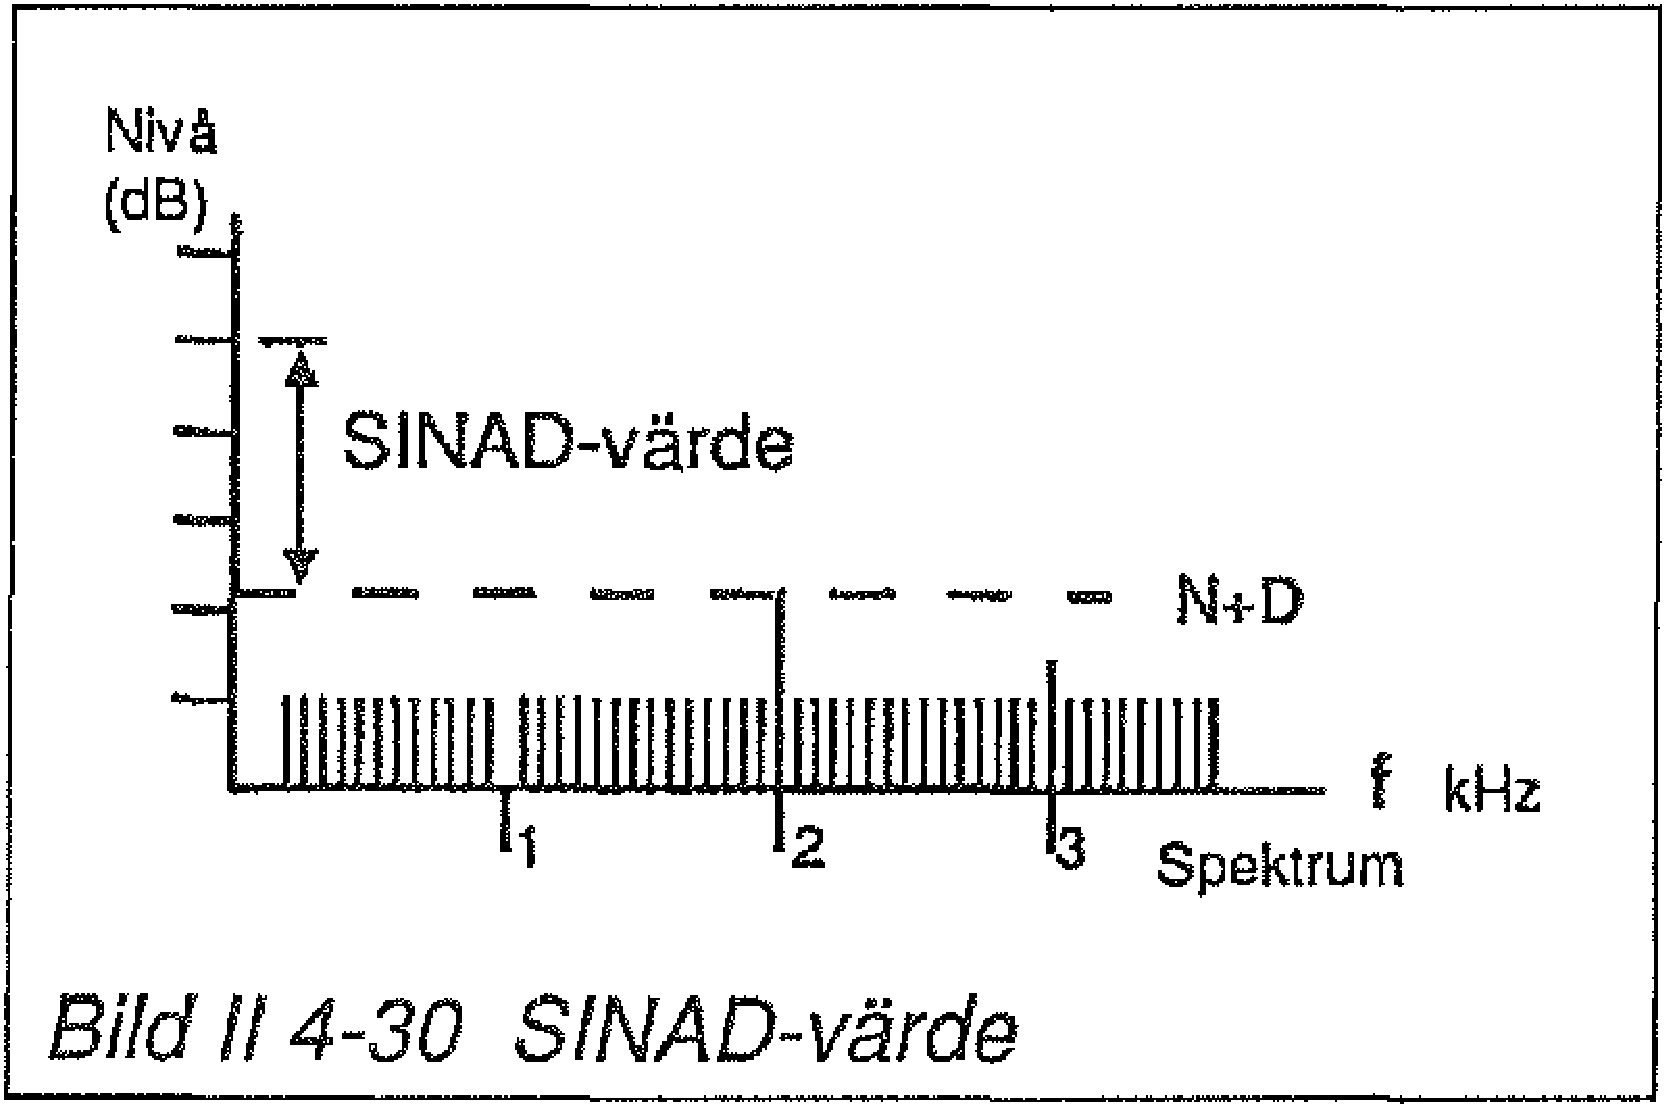
\includegraphics[width=0.5\textwidth]{images/bild_2_4-30}
  \caption{SINAD-värde}
  \label{fig:bildII4-30}
\end{wrapfigure}

I en broschyr på en kortvågsmottagare kan man t.ex. läsa
''Sensitivity SSB, CW: less than 0,25~µV for 10~dB S/N''

Termen S/N betyder Signal/Noise, d.v.s. styrkeförhållandet signal/brus
uttryckt i dB. Det innebär att en signal kan läsas vid 25~µV signalnivå
och ett S/N av mindre än 10~dB.
Utöver brusnivån i mottagaren spelar också distorsionen en roll.

\begin{align*}
  \begin{array}[b]{l}
    \text{Signalbrus-} \\
    \text{förhållande}
  \end{array} &= \frac{S + N + D}{N} \text{ dB} \\
  \text{där} \quad S &= \text{Signalnivå} \\
  N &= \text{Brusnivå} \\
  D &= \text{Distorsionsnivå} \\
\end{align*}

I en broschyr på en VHF-mottagare kan man t.ex. läsa
''Sensitivity FM: Less than 0,18~µV for 12~dB SINAD''

Termen SINAD betyder Signal, Noise and Distorsion. Vid denna
definition tar man även hänsyn till distorsionsprodukter som orsakas
av den modulerande signalen. 

\[
\text{SINAD} = \frac{S+N+D}{N+D}\text{ dB}
\]

\subsection{Intermodulation, korsmodulation}
\textbf{HAREC a.\ref{HAREC.a.4.4.6}\label{myHAREC.a.4.4.6}}
\index{intermodulation}
\index{korsmodulation}

Utöver att en bra modern mottagare bör ha tillräcklig
frekvensstabilitet, känslighet och selektivitet bör den även ha goda
s.k. storsignalegenskaper.

Med storsignalegenskaper menar man hur bra en relativt svag
nyttosignal på mottagaringången motstår påverkan av starka
frekvens nära signaler med hög fältstyrka. Störningar av detta slag
uppstår genom icke linjära förlopp i komponenter i mottagarens
ingångssteg, varvid mottagna signaler med stor amplitud blir
förvrängda.

Korsmodulation och intermodulation är två begrepp som är förknippade
med storsignalegenskaperna. Båda kan visserligen definieras och
bestämmas entydigt, men de förväxlas ändå ofta.

\subsubsection{Korsmodulation}
\index{korsmodulation}
\index{mottagare!korsmodulation}

Med korsmodulation menas, att den inkommande nyttosignalen
amplitudmoduleras med modulationsprodukter från en annan frekvensnära
amplitudmodulerad signal, varvid korsmodulationen uppstår i olinjära
komponenter i mottagaringången (försteg, blandare). När man med
mottagaren i AM-läge ställt in den på någon bärvåg så hörs också andra
starka, frekvensnära stationer.

Det måste alltså alltid finnas en nyttosignal på den inställda
frekvensen för att det ska uppstå korsmodulation. När nyttosignalen
försvinner så försvinner även korsmodulationen.

\subsection{Intermodulation}
\index{intermodulation}
\index{mottagare!intermodulation}

Vid s.k. intermodulation blandas två starka inkommande signaler i
olinjära komponenter i mottagaringången. Deras blandningsprodukter
faller på mottagningsfrekvensen så att den störs, vare sig det finns
en nyttosignal där eller inte.

\subsection{Frekvensstabilitet}

Se avsnitt \ref{oscillatorer}.
